
\begin{frame}{Realidad Virtual - Antecedente hist\'orico}

\begin{columns}
\begin{column}{0.49\textwidth}


\begin{itemize}
\item Un estereoscopio proporciona im\'agenes separadas para cada ojo mediante lentes individuales, donde cada imagen tiene una variante en el angulo de captura y un desplazamiento horizontal.
\item El cerebro de una persona con una percepción binocular normal de la profundidad al utilizar el estereoscopio ``mezcla'' ambas imagenes para crear una  ``ventana estereoscópica''
\end{itemize}
\end{column}

\begin{column}{0.49\textwidth}

\begin{center}
	\begin{tabular}{cc}
        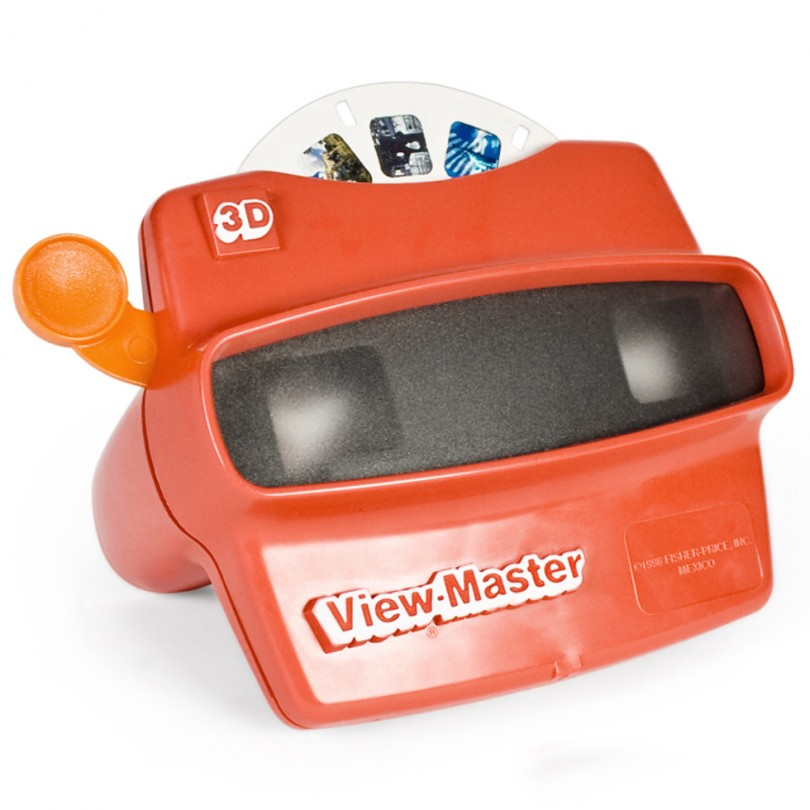
\includegraphics[width=0.45\linewidth]{Figs/view_master_blog-810x810.jpg} &
		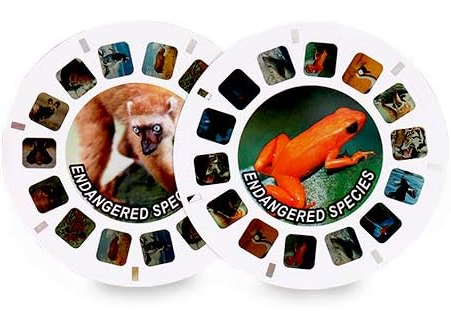
\includegraphics[width=0.45\linewidth]{Figs/DiscosViewMaster.png}    
	\end{tabular}

	\begin{tabular}{cc}
	\centering
        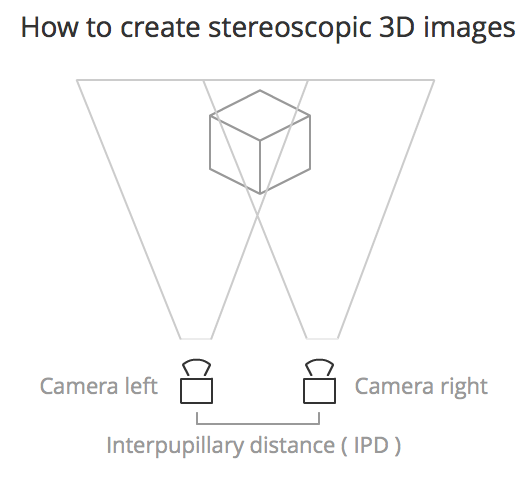
\includegraphics[width=0.49\linewidth]{Figs/VirtualReal1} &
        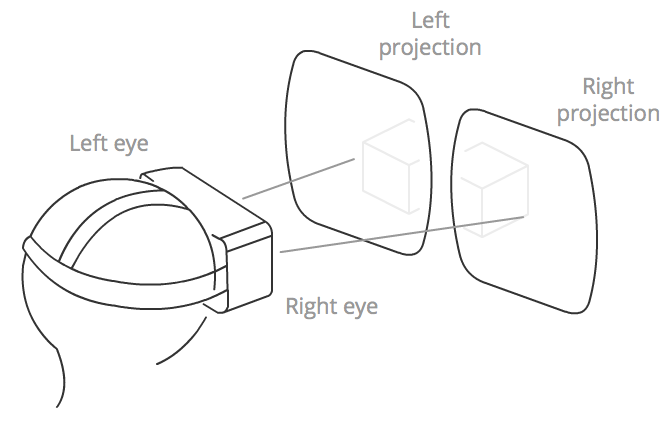
\includegraphics[width=0.49\linewidth]{Figs/VirtualReal2} \\

	\end{tabular}
\end{center}
\end{column}

\end{columns}
	
\end{frame}




\begin{frame}{Realidad Virtual (VR)}
%\begin{block}{Realidad Virtual (VR)} 
		\begin{itemize}
			\item La Realidad virtual (RV) emplea modelos y simulaciones por computadora que permite a una persona interactuar con un entorno visual artificial tridimensional (3D)
			\item En un formato típico de RV, un usuario lleva un casco con una pantalla estereoscópica para ver imágenes animadas de un entorno simulado
			\item El dispositivo m\'as econ\'omico para aplicaciones de RV es un tel\'efono inteligente 
		\end{itemize}
    \begin{center}
	\begin{tabular}{ccc}
    	\centering
		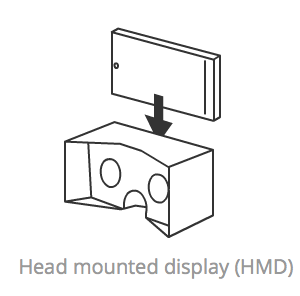
\includegraphics[width=0.25\linewidth]{Figs/MobileVR2} & 
        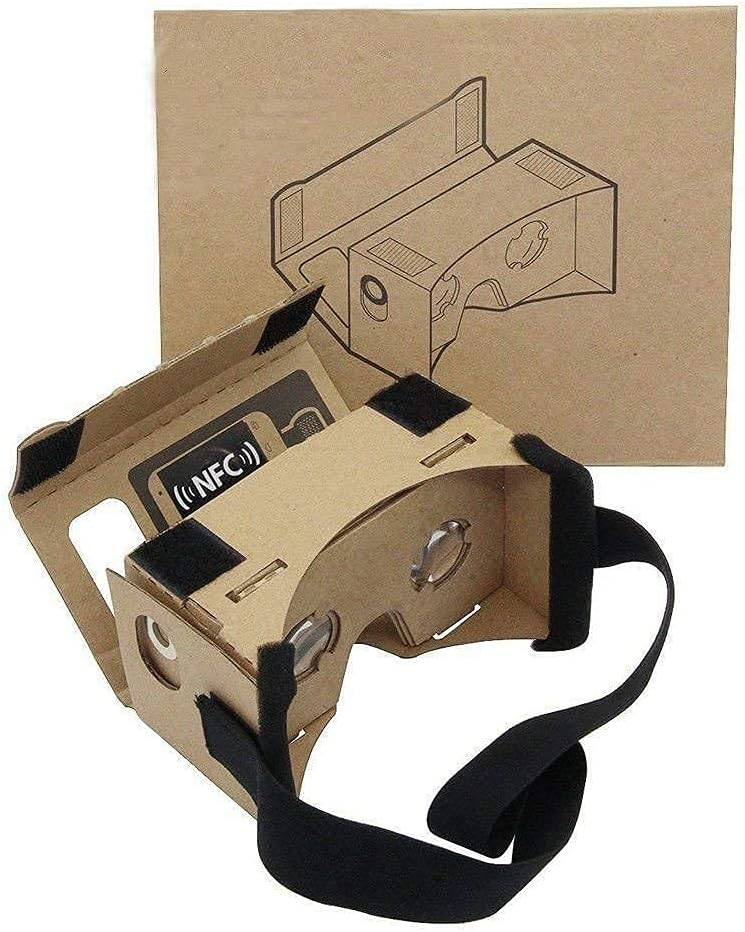
\includegraphics[width=0.19\linewidth]{Figs/CardBoard} & 		
        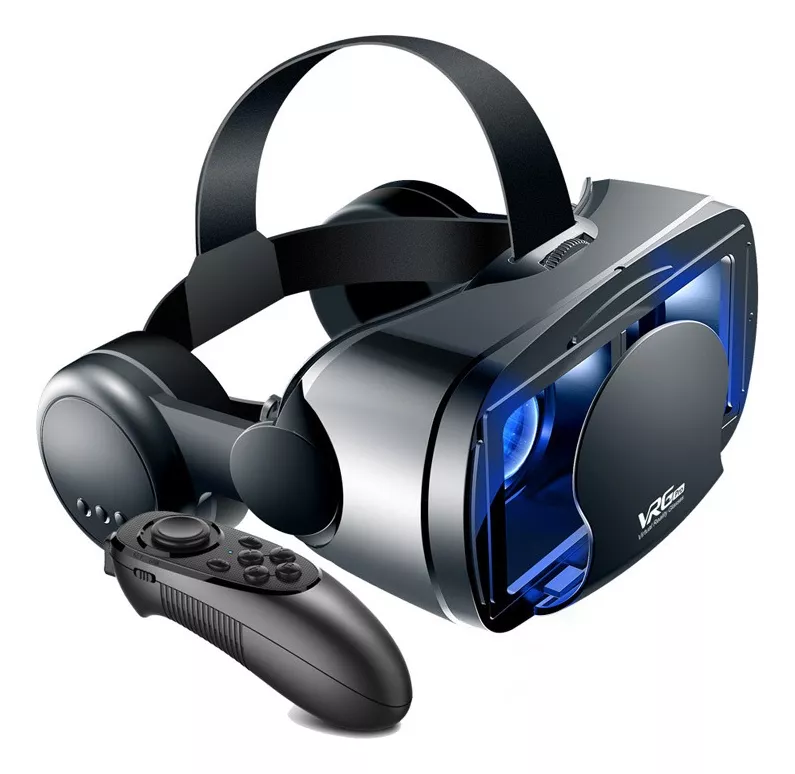
\includegraphics[width=0.19\linewidth]{Figs/VRGPro} 		
	\end{tabular}
		 \end{center}
%\end{block} 
\footnotetext{\url{https://reference.codeproject.com/book/dom/webvr_api/webvr_concepts}}
\end{frame}


\begin{frame}{Costos de Dispostivos HeadSets para VR}
\begin{columns}
\begin{column}{0.49\textwidth}
\begin{itemize}
\item Meta Quest 3 (499 USD)
\item Sony PlayStation VR2 (599 USD)
\item Meta Quest Pro (900 USD)
\item Valve Index VR Kit (1350 USD)
\item HTC Vive Pro 2 (1400 USD)
\end{itemize}

\begin{center}
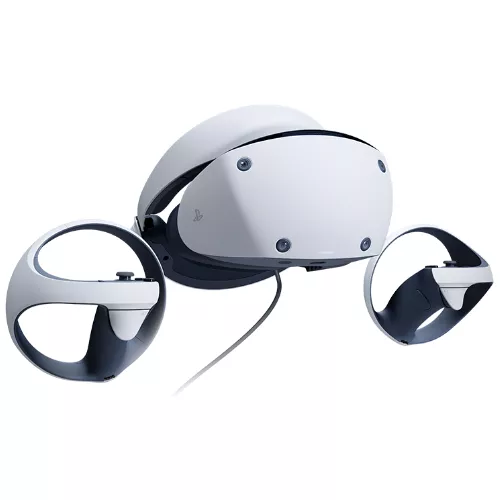
\includegraphics[width=0.75\textwidth]{Figs/sony.png}
\end{center}
\end{column}
\begin{column}{0.49\textwidth}
\begin{center}
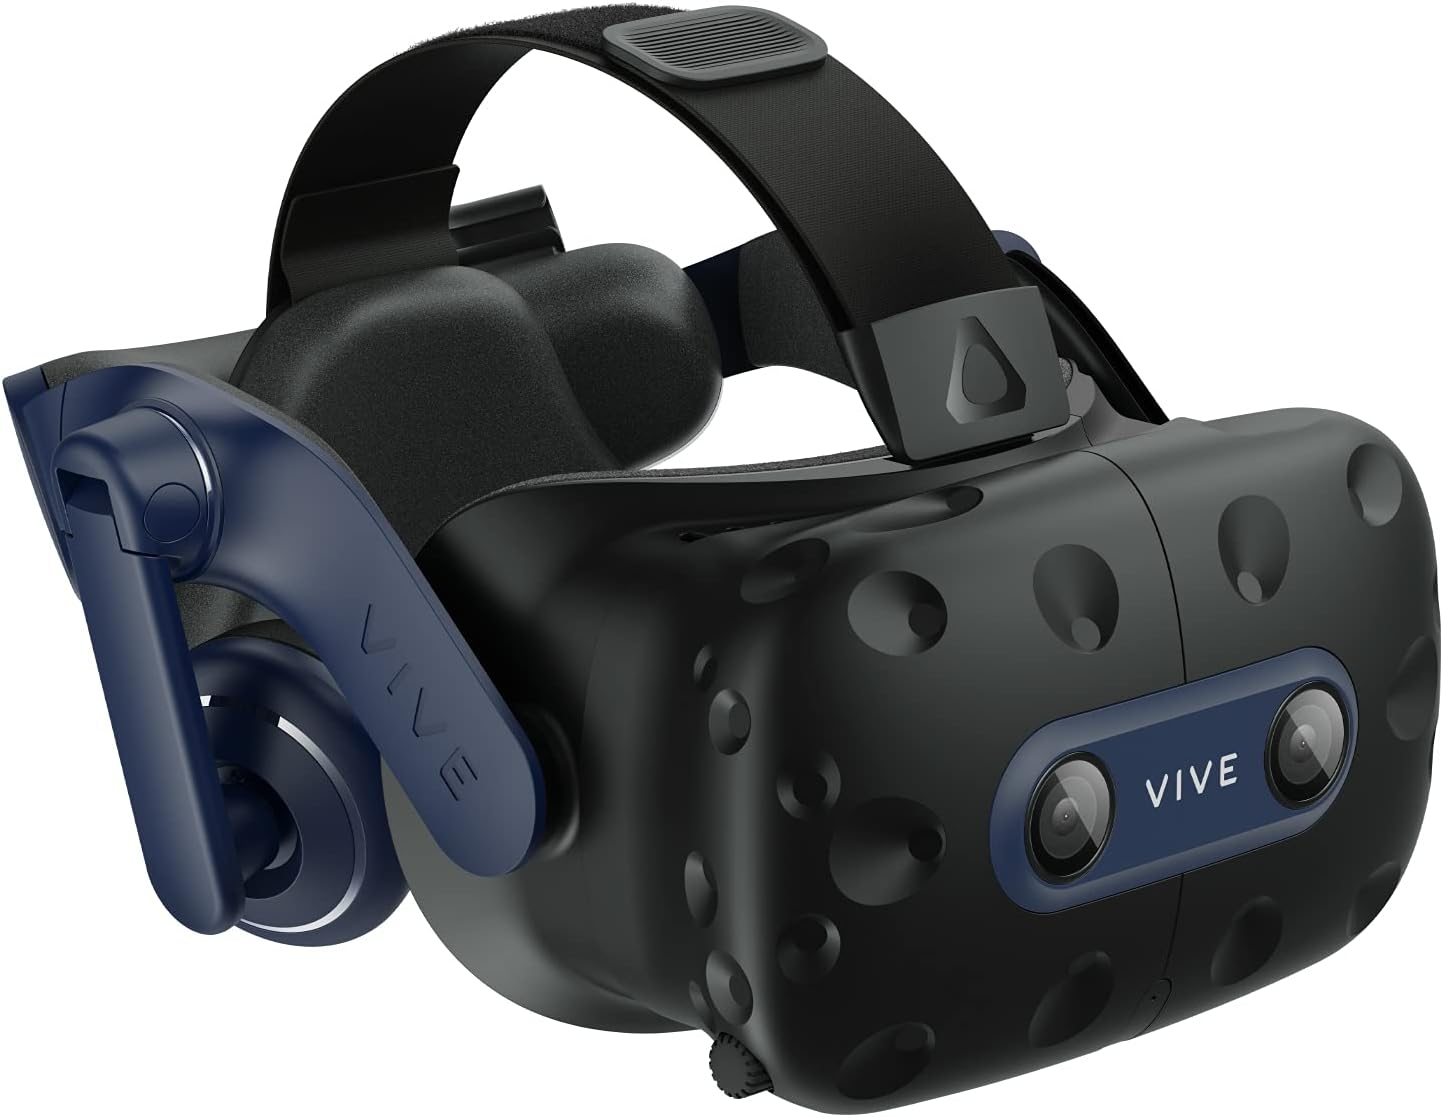
\includegraphics[width=0.75\textwidth]{Figs/HTC.jpg}\\
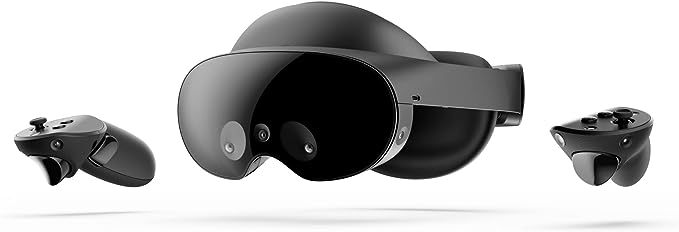
\includegraphics[width=0.95\textwidth]{Figs/MetaPro.jpg}
\end{center}
\end{column}
\end{columns}
\end{frame}


\begin{frame}{Relación entre RV - Teléfonos Inteligentes}
Los teléfonos inteligentes son una de las principales plataformas para sistemas de realidad virtual (VR):  
\begin{itemize}
\item Tienen hardware avanzado (cámaras, sensores de movimiento, procesadores gráficos) que permiten ejecutar experiencias inmersivas de VR sin necesidad de equipos especializados.  
\item Existen accesorios como \textbf{gafas VR para móviles} (ej. Google Cardboard, Samsung Gear VR) que convierten un teléfono en un visor de realidad virtual.  
\item Existen herramientas para crear apps de  RV
\item Muchas aplicaciones combinan AR con inteligencia artificial para ofrecer experiencias interactivas y personalizadas.  
\item Gran cantidad de aplicaciones prácticas
\end{itemize}
\end{frame}
